\section{Punto de Vista de Producto}


\subsection{Modelo de Producto}
\begin{figure}[h!]
	\centering
	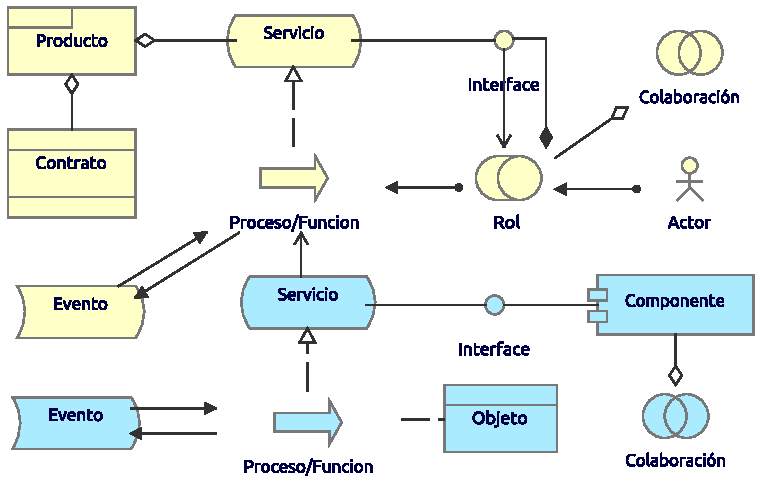
\includegraphics[width=.6\linewidth]{imgs/modelo/Producto.pdf}
	\caption{Modelo Producto}
\end{figure}

El punto de vista de producto permite ver el conjunto de contratos que rigen un producto de la organización, además relaciona los servicios que se desprenden del producto. Estos contratos son aquello que regulan y limitan  al producto. Los servicios asociados al producto son parte de los objetivos, misión y visión de la empresa y que desembocan en proceso de la organización ya sea implícito o explícito relacionado obviamente con el producto.

\newpage
\subsection{Caso  de Producto}
\begin{figure}[h!]
	\centering
	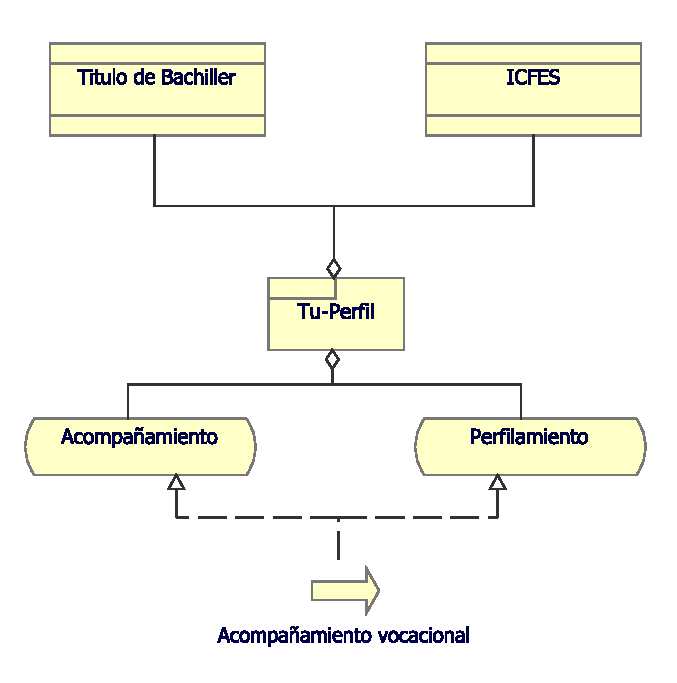
\includegraphics[width=.9\linewidth]{imgs/caso/negocio/producto.pdf}
	\caption{Caso Producto}
\end{figure}

Para el caso de estudio tenemos como producto de negocio a Tu-Perfil aquel apartado que servirá como guiá para acompañar y perfilar a los estudiantes en la elección de vocación que sera tomada al graduarse como bachiller con el fin de dar cabida al proceso de acompañamiento vocacional que surge de los objetivos de la organización para este caso el MEN.  Este producto esta regido por los contratos definidos ICFES y Titulo de Bachiller, que serán aquellos que limitaran al producto.